\documentclass{beamer}
\usepackage[T2A]{fontenc}
\usepackage[utf8x]{inputenc}
\usepackage[english,russian]{babel}
\usepackage{amssymb,amsfonts,amsmath,mathtext}
\usepackage{cite,enumerate,float,indentfirst}
\usepackage{listingsutf8}
\usepackage{listings}
\definecolor{light-gray}{gray}{0.95}
\PrerenderUnicode{Рҷ}
\lstset{
  inputencoding=utf8x,
  extendedchars=\true,
  showstringspaces=false,
  basicstyle=\ttfamily\tiny,
  tabsize=2,
  backgroundcolor=\color{light-gray},
}
\usetheme[pageofpages=из,% String used between the current page and the
                         % total page count.
          bullet=circle,% Use circles instead of squares for bullets.
          titleline=true,% Show a line below the frame title.
          alternativetitlepage=false,% Use the fancy title page.
          titlepagelogo=logo-polito,% Logo for the first page.
          watermark=,% Watermark used in every page.
          watermarkheight=100px,% Height of the watermark.
          watermarkheightmult=4,% The watermark image is 4 times bigger
                                % than watermarkheight.
          ]{Torino}
\usecolortheme{nouvelle}
\author{Османов А.Л.}
\title{СОЗДАНИЕ RDF-ХРАНИЛИЩА ИНФОРМАЦИИ НА РУССКОМ ЯЗЫКЕ ПО ЛЕКАРСТВЕННЫМ ПРЕПАРАТАМ}
\institute{Кафедра технологий программирования \\ Научный руководитель: доктор физико-математических наук, профессор Соловьев В.Д.}

\date{Казань \\ 2012}


\begin{document}
% DO NOT COMPILE THIS FILE DIRECTLY!
% This is included by the other .tex files.

\begin{frame}[t,plain]
\titlepage
\end{frame}

\begin{frame}[t]{Преимущества Semantic Web}
\begin{tabular}{l l}
\begin{minipage}{0.5\textwidth}
\begin{itemize}
\item Легкий обмен информацией между хранилищами знаний.
 \vspace{1em}
\item Извлечение релевантной информации для поисковых систем. 
 \vspace{1em}
\item Получение нового знания.
 \vspace{1em}
\item Интеграция в мировое распределенное хранилище знаний.
\end{itemize}
\end{minipage}
&
\begin{minipage}{0.5\textwidth}

\includegraphics[width=15mm]{link.png}
\\
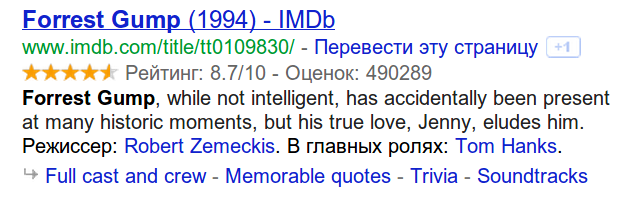
\includegraphics[width=50mm]{imdb.png}
\\

\includegraphics[width=15mm]{sparql.png}
\\
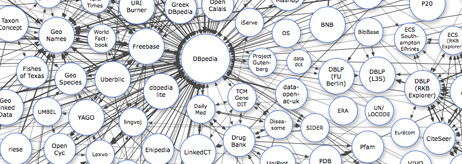
\includegraphics[width=50mm]{semwebgraph.png}
\end{minipage}
\end{tabular}

\end{frame}

\begin{frame}[t,fragile]{Используемые технологии}

\includegraphics[width=100mm]{words.png}
\end{frame}
\begin{frame}[t]{Онтология}
  \begin{itemize}
  \item Описывание взаимоотношений.
    \\Лекарство:
    \begin{itemize}
    \item ...
    \item имеет международное название
    \item имеет торговое наименование
    \item принадлежит нескольким категориям
    \item имеет множество форм применения
    \item имеет множество показаний
    \item имеет множество противопоказаний
    \item имеет множество побочных эффектов
    \item взаимодействует с другими лекарствами и группами лекарств
    \item содержит лекарственные ингридиенты
    \item ...
    \end{itemize}
  \item Protege
  \end{itemize}
\end{frame}
\begin{frame}[t]{Онтология}

\begin{tabular}{l l}
\begin{minipage}{0.6\textwidth}
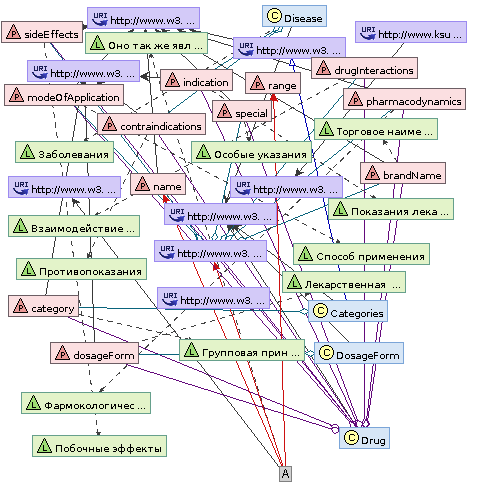
\includegraphics[width=70mm]{onto.png}
\end{minipage}
&
\begin{minipage}{0.4\textwidth}
\begin{itemize}
\item Информация о данных в RDF-хранилище
\item Взаимоотношения между отношениями
\end{itemize}
\end{minipage}
\end{tabular}
\end{frame}
\begin{frame}[t]{Выбор RDF-хранилища}
 \begin{itemize}
  \item 3store
  \item Sesame
  \item RDFdo
  \item Jena
 \end{itemize}
\end{frame}
\begin{frame}[t]{Сравнение RDF-хранилищ}
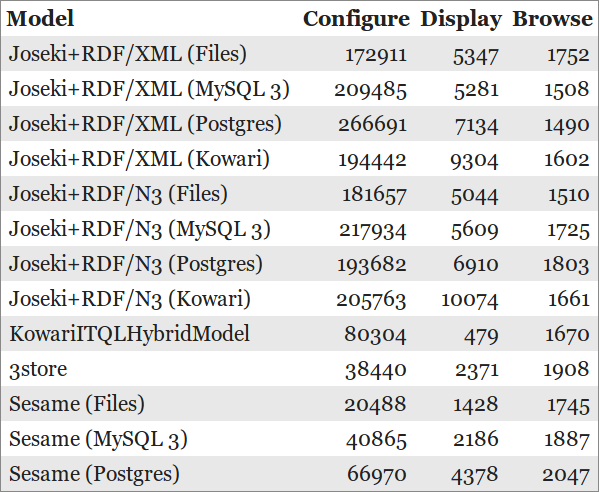
\includegraphics[width=70mm]{storages.png}
\end{frame}
\begin{frame}[t]{Парсинг ресурса Webapteka.ru}
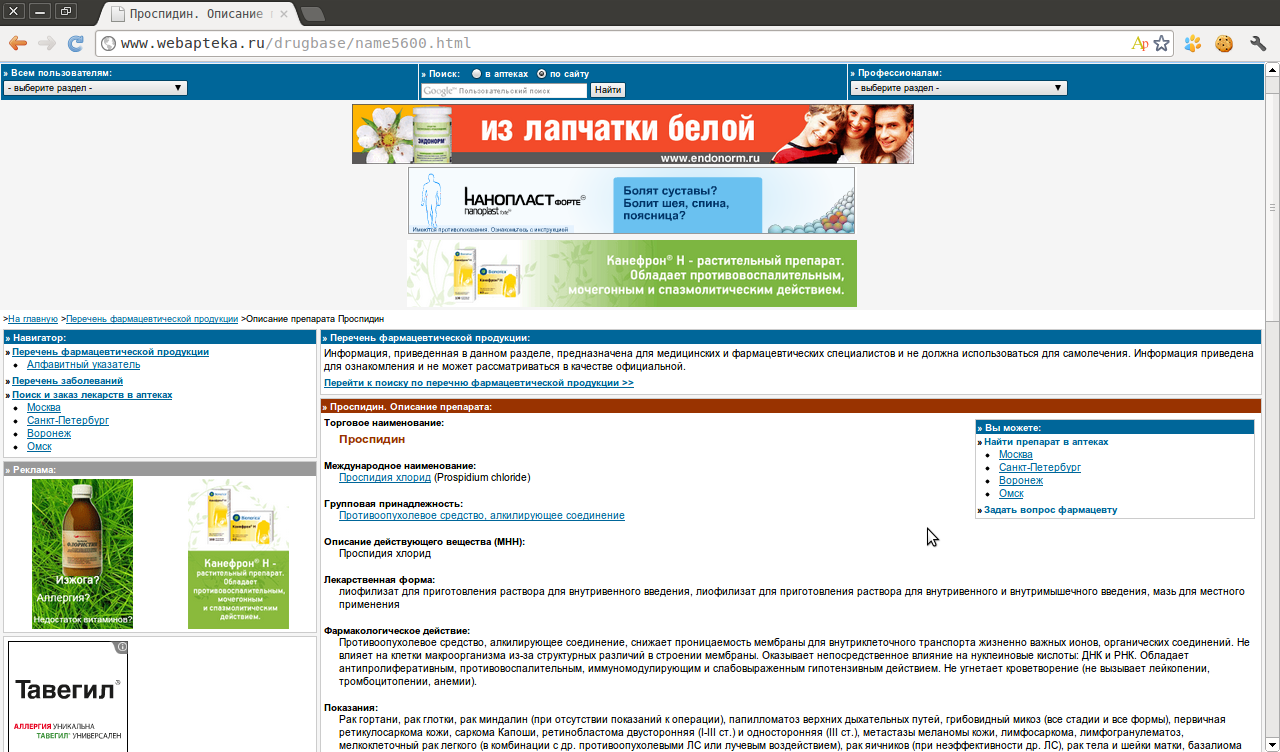
\includegraphics[width=100mm]{webapteka.png}
\end{frame}
\begin{frame}[fragile]{Spira}
\begin{lstlisting}
type URI.new("http://osmanov.me/drugs")

property :brandName,  
  :predicate => FOAF.name, 
  :type => String
has_many :drugCategories, 
  :predicate => URI.new("http://osmanov.me/has_drug_category"), 
  :type => :DrugCategory

has_many :contraindications, 
  :predicate => URI.new("http://osmanov.me/has_contraindication"), 
  :type => String
\end{lstlisting}
\begin{lstlisting}[language=Ruby]
drug.brandName = "Аспирин"
\end{lstlisting}
\end{frame}
\begin{frame}[t]{RDF-граф}

\begin{tabular}{l l}
\begin{minipage}{0.75\textwidth}
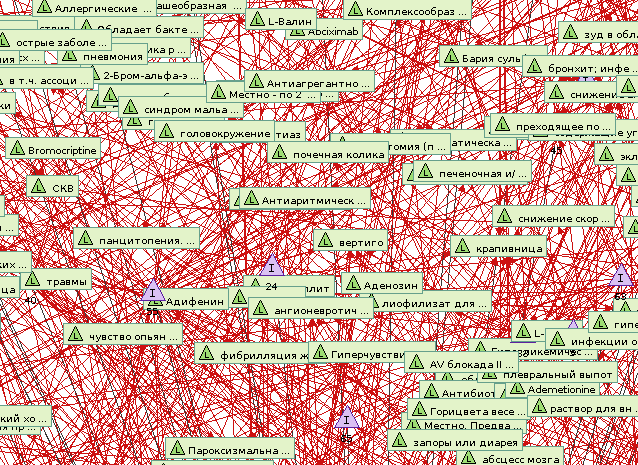
\includegraphics[width=80mm]{graph.png}
\end{minipage}
&
\begin{minipage}{0.25\textwidth}
\begin{itemize}
\item 20000 лекарств
\item 1180000 триплетов
\end{itemize}
\end{minipage}
\end{tabular}
\end{frame}
\begin{frame}[fragile]{SPARQL}
Похожие лекарства
\begin{lstlisting}
  SELECT ?drug 
  WHERE {
    ?drug <http://osmanov.me/drugComponent> ?drugPart .
    <#{uri}> <http://osmanov.me/drugComponent> ?drugPart
    FILTER (?drug != <#{uri}>)
  }
\end{lstlisting}
Суммарные противопоказания
\begin{lstlisting}
  SELECT ?contraindication
  WHERE {
	  #{names_query} .
	  ?drug <http://osmanov.me/has_contraindication> ?contraindication
  }
\end{lstlisting}


\end{frame}


\end{document}

